\documentclass[12pt, a4paper]{exam}

\usepackage[utf8]{inputenc}
\usepackage[T1]{fontenc}
\usepackage[french]{babel}
\usepackage{listings}
\usepackage{hyperref}
\usepackage{graphicx}
\usepackage{lastpage}

\pagestyle{headandfoot}

\firstpageheader{BTS CIEL1}{Évaluation pratique : Programmation orientée objet}{27/04/2026}

\runningfooter{BTS CIEL 1}
{Page \thepage\ sur \numpages}
{27/04/2026}

\begin{document}
\pagenumbering{arabic}

\begin{center}
  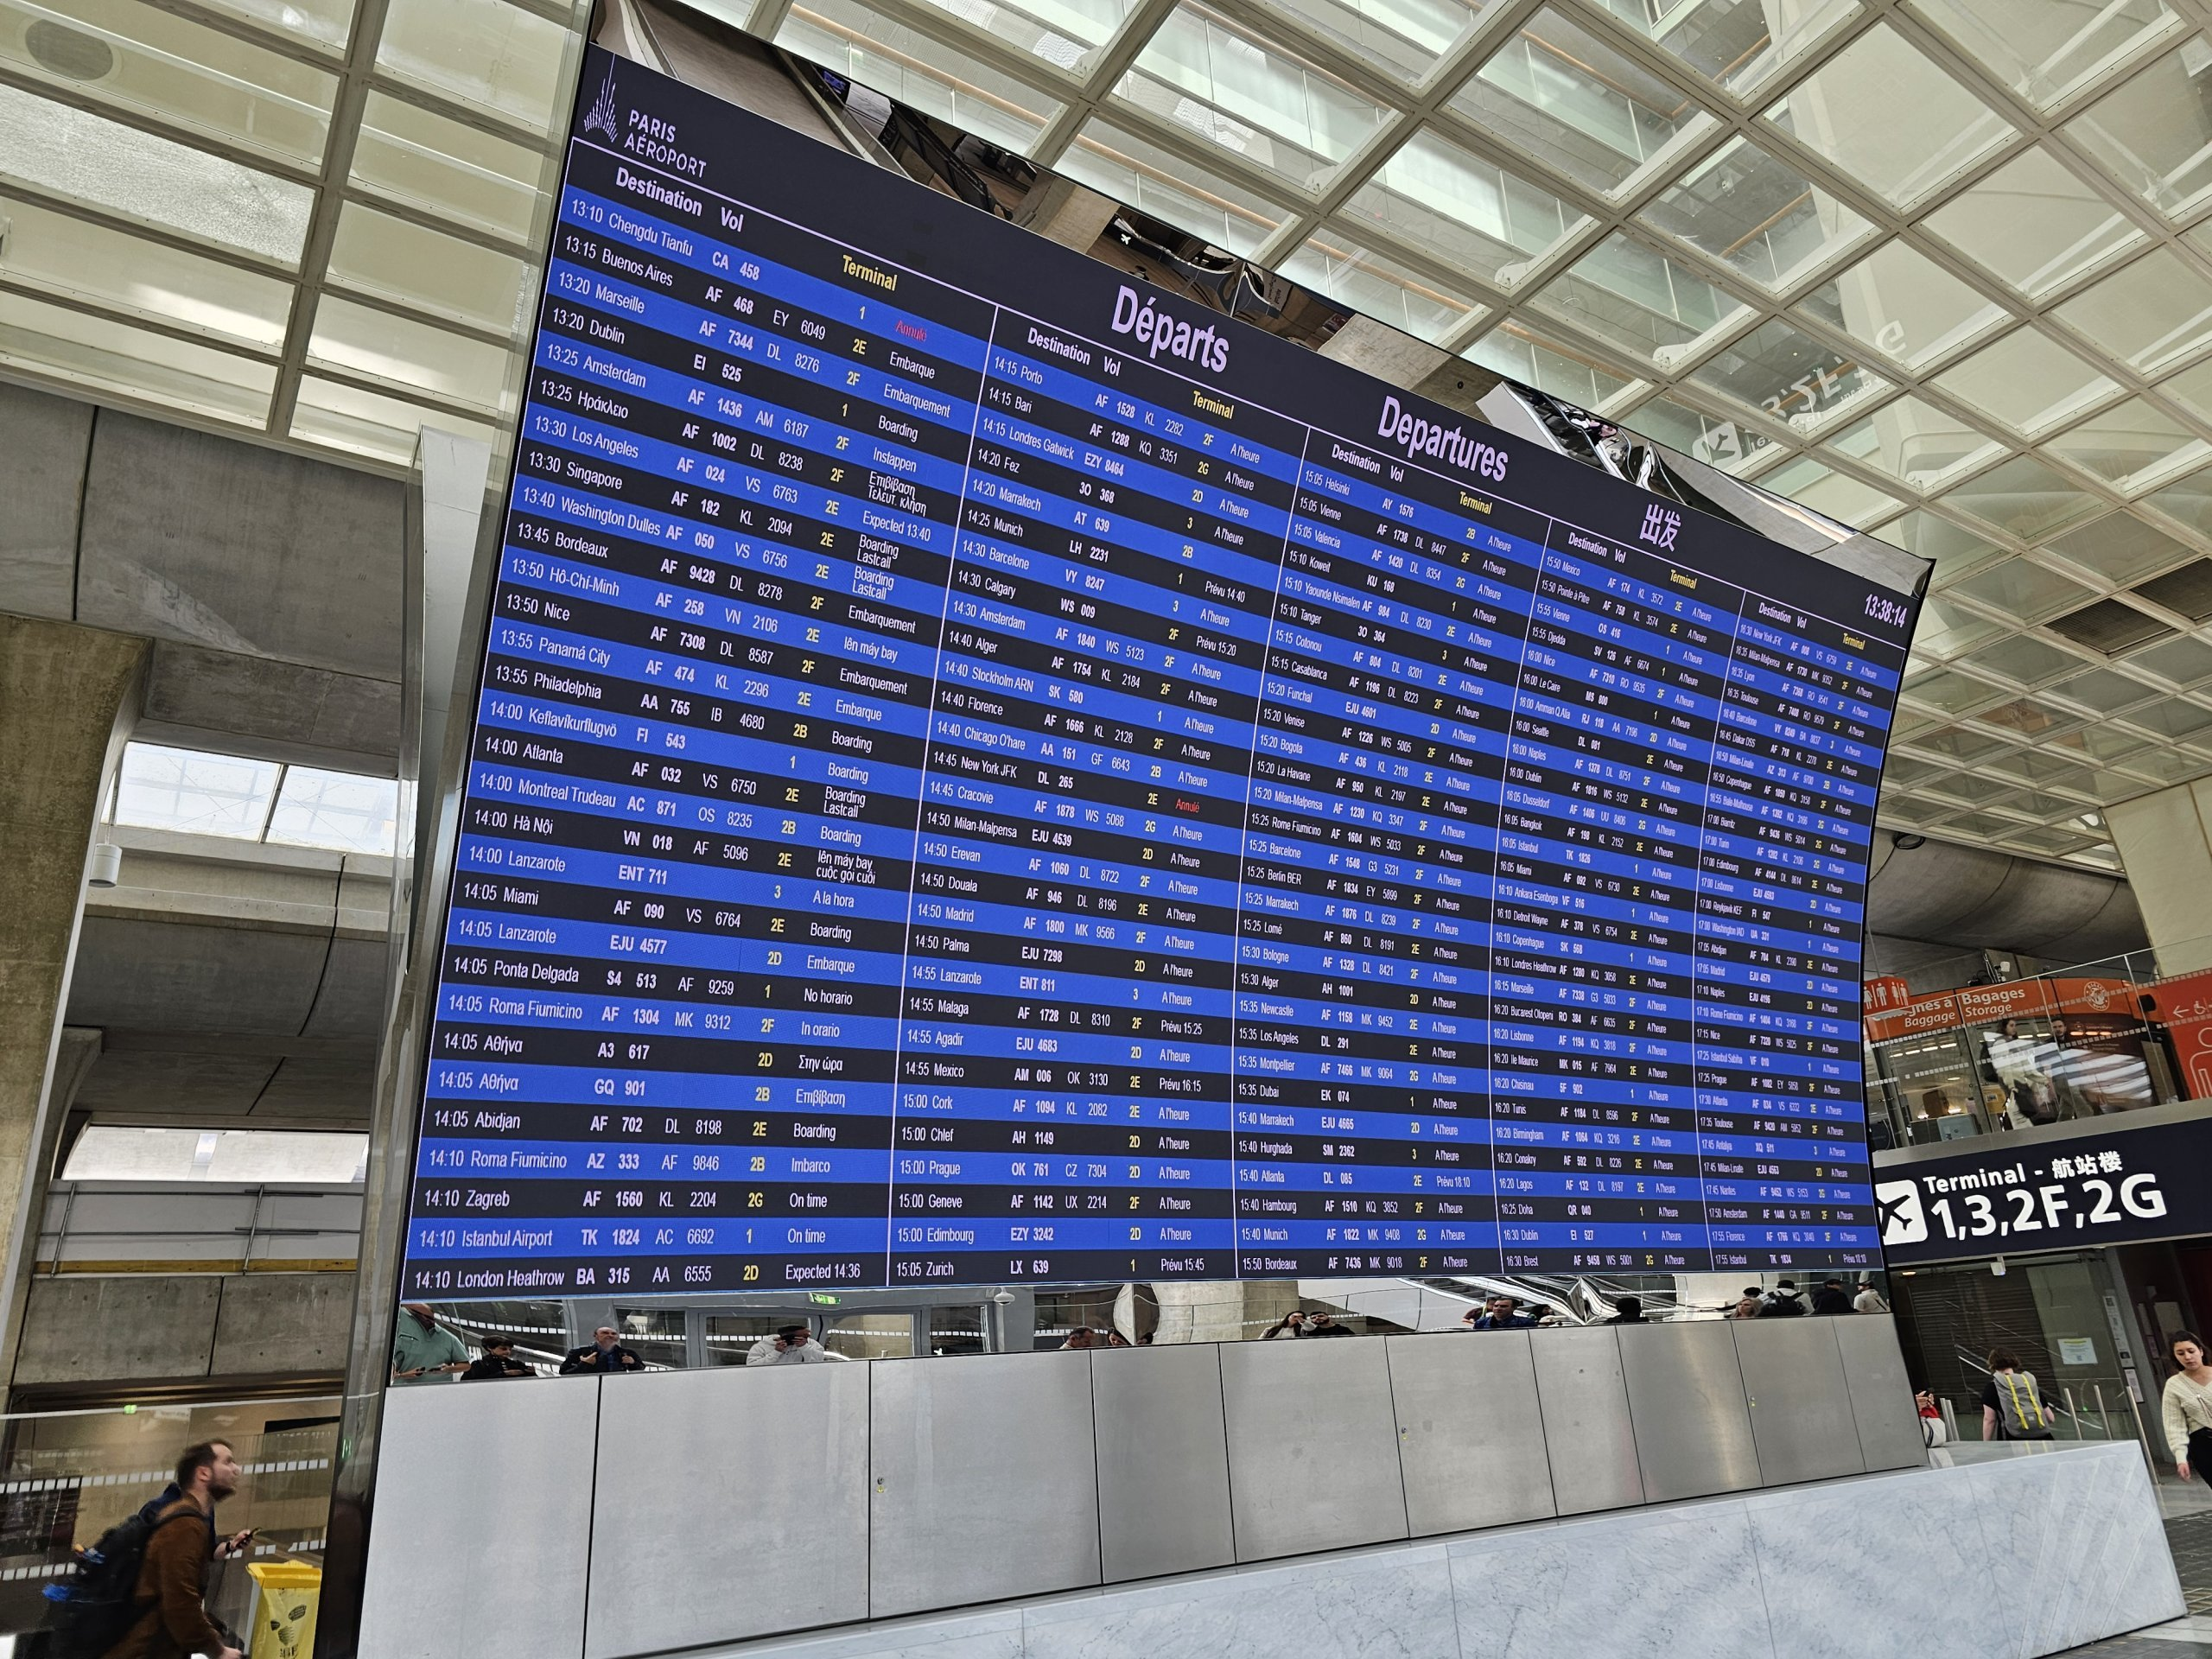
\includegraphics[width=200px]{CDG_departures.jpeg}
\end{center}
\begin{center}
Nom et prénom:\enspace \hrulefill \hfill Note :\enspace \hrulefill
\end{center}

\section{Contexte}

L'organisation d'un aéroport est un processus complexe qui implique la coordination de nombreux éléments pour assurer le bon déroulement des opérations. Parmi les aspects cruciaux de cette organisation, la gestion des retards de départs des vols occupe une place centrale. Les retards peuvent être causés par divers facteurs tels que les conditions météorologiques, les problèmes techniques, les contraintes de trafic aérien, ou encore les retards accumulés lors des vols précédents. La capacité à analyser et à gérer efficacement ces retards est essentielle pour minimiser les impacts sur les passagers, les compagnies aériennes, et les opérations aéroportuaires dans leur ensemble.

La société EUROCONTROL étudie la performance des aéroports européens et met à disposition des jeux de données (disponible ici : \url{https://ansperformance.eu/data/}) contenant différentes métriques permettant de comparer les aéroports sur différentes thématiques :
\begin{itemize}
  \item L'impact environnemental (émissions CO\textsubscript{2}, NO\textsubscript{x} et SO\textsubscript{x})
  \item L'efficacité opérationnelle (gestion du trafic aérien terminal et en route)
  \item La performance économique (coûts et investissements des systèmes de contrôle aérien)
\end{itemize}

L'objectif de ce TP est de réaliser un programme Python permettant d'extraire les informations d'un fichier contenant le nombre de vols opérés pour chaque aéroport par mois depuis le début de l'année ainsi que le cumul des retards.

Le programme permettra à l'utilisateur de saisir un identifiant d'aéroport (code ICAO), un mois et une année afin de connaître le nombre de vols et le cumul de retard associés.

Les fichiers à votre disposition sont :

\begin{itemize}
  \item \texttt{all\_pre\_departure\_delays\_2026.csv} contenant le nombre de vols opérés par aéroport par mois sur l'année 2026 ainsi que le cumul des retards
  \item \texttt{main.py} contenant le programme que vous devez compléter
\end{itemize}

\section{Exemple}

Voici un exemple de contenu du fichier \texttt{all\_pre\_departure\_delays\_2026.csv} :

\begin{verbatim}
YEAR,MONTH_NUM,MONTH_MON,FLT_DATE,APT_ICAO,APT_NAME,STATE_NAME,
FLT_DEP_1,FLT_DEP_IFR_2,DLY_ALL_PRE_2
2026,01,JAN,2026-01-01,LFMH,Saint-Etienne-Boutheon,France,0,,
2026,01,JAN,2026-01-01,LFML,Marseille-Provence,France,101,101,1524
2026,01,JAN,2026-01-01,LFMN,Nice-Cote d'Azur,France,136,136,1765
2026,01,JAN,2026-01-01,LFMP,Perpignan-Rivesaltes,France,5,,
2026,01,JAN,2026-01-01,LFMT,Montpellier-Mediterranee,France,16,,
2026,01,JAN,2026-01-01,LFMU,Beziers-Vias,France,1,,
2026,01,JAN,2026-01-01,LFMV,Avignon-Caumont,France,1,,
2026,01,JAN,2026-01-01,LFOB,Beauvais-Tille,France,50,,
2026,01,JAN,2026-01-01,LFOK,Chalons-Vatry,France,1,,
2026,01,JAN,2026-01-01,LFOT,Tours-Val de Loire,France,1,,
2026,01,JAN,2026-01-01,LFPB,Paris - Le Bourget,France,31,,
2026,01,JAN,2026-01-01,LFPG,Paris - Charles-de-Gaulle,France,594,599,13453
\end{verbatim}

En prenant la dernière ligne, il s'agit de l'aéroport de Paris-Charles-de-Gaulle (LFPG ou code IATA CDG) : sur le mois de janvier 2026, il a opéré 594 vols et cumulé 13\,453 minutes de retard (soit plus de 224 heures).

La signification des champs est la suivante :

\begin{itemize}
  \item \texttt{YEAR} / \texttt{MONTH\_NUM} / \texttt{MONTH\_MON} : année, numéro et nom du mois
  \item \texttt{FLT\_DATE} : date d'observation (souvent à l'échelle du jour)
  \item \texttt{APT\_ICAO} : code ICAO de l'aéroport (identifiant unique, ex : LFPG)
  \item \texttt{APT\_NAME} : nom de l'aéroport
  \item \texttt{STATE\_NAME} : pays de l'aéroport
  \item \texttt{FLT\_DEP\_1} : nombre total de départs via NM (gestionnaire du réseau)
  \item \texttt{FLT\_DEP\_IFR\_2} : nombre de départs via APT (opérateur de l'aéroport)
  \item \texttt{DLY\_ALL\_PRE\_2} : total des retards cumulés (en minutes, source 2)
\end{itemize}

Les variables \texttt{FLT\_DEP\_1} et \texttt{FLT\_DEP\_IFR\_2} mesurent toutes deux les départs, mais selon des sources différentes. Les écarts éventuels entre ces colonnes reflètent des différences de méthode de comptage et de consolidation des données. Dans notre cas, nous utiliserons uniquement \texttt{FLT\_DEP\_1}.

\newpage
\section{Etapes}

\textit{\textbf{Vous devez faire valider chaque étape avant de passer à la suivante}}.

\textit{\textbf{Des commentaires dans le code vous indiquent les parties à compléter}}.

\begin{questions}

  \question[5]{Ouverture du fichier et chargement des données}

  Dans la fonction \texttt{main}, implémentez l'ouverture du fichier CSV et le chargement
  des données dans la liste \texttt{delays\_and\_departures}.

  Le programme devra :
  \begin{itemize}
    \item Ouvrir le fichier \texttt{all\_pre\_departure\_delays\_202.csv} en lecture
    \item Ignorer la première ligne d'en-tête
    \item Lire chaque ligne du fichier et extraire les champs utiles
    \item Créer un objet \texttt{AirportDepartureDelay} pour chaque ligne
    \item Ajouter chaque objet à la liste \texttt{delays\_and\_departures}
    \item Gérer le cas où le fichier est absent avec un message d'erreur adapté
  \end{itemize}

  \question[4]{Compléter la classe \texttt{AirportDepartureDelay}}

  Complétez la classe \texttt{AirportDepartureDelay} en implémentant les parties manquantes :
  \begin{itemize}
    \item Initialisation des attributs manquants dans le constructeur
    \item Calcul de la moyenne des retards dans \texttt{mean\_delay}
    \item Représentation textuelle de l'objet dans \texttt{\_\_repr\_\_}
  \end{itemize}

  \question[4]{Saisie utilisateur et gestion des erreurs}

  Demandez à l'utilisateur :
  \begin{itemize}
    \item Le code de l'aéroport (3 ou 4 lettres, ex : LFPG)
    \item L'année (4 chiffres)
    \item Le mois (un entier de 1 à 12)
  \end{itemize}

  Assurez-vous de gérer les erreurs de saisie (format incorrect, valeurs hors limites) avec des messages d'erreur clairs et une nouvelle demande de saisie.

  \question[2]{Modifier le comportement du tri}

  Modifiez les méthodes \texttt{\_\_lt\_\_}, \texttt{\_\_gt\_\_} et \texttt{\_\_eq\_\_}
  de la classe \texttt{AirportDepartureDelay} afin d'adapter le comportement de
  \texttt{sort()} sur la liste des objets.

  \question[2]{Expliquer un extrait de code}

  Expliquez le rôle du code suivant dans le constructeur de la classe \texttt{AirportDepartureDelay} du fichier \texttt{main.py} :
  \begin{verbatim}
  if self.to_month < self.from_month :
    self.to_year = self.from_year + 1
  else:
    self.to_year = self.from_year
  \end{verbatim}

  \response[2cm]

  \question[2]{Ajouter un cumul depuis le début de l'année}

  Écrivez une fonction qui regroupe les retards et le nombre de vols d'un même aéroport
  depuis le début de l'année. Le programme doit ensuite permettre à l'utilisateur de
  demander ce cumul depuis le début de l'année.

\end{questions}

\end{document}
